\chapter{Kravspecifikation}

\begin{longtabu} to \linewidth{@{}l l l X[j]@{}}
    Version &    Dato &    Ansvarlig &    Beskrivelse\\[-1ex]
    \midrule

\label{version_Systemark}
\end{longtabu}


\section{Indledning}


\section{Funktionelle krav}
De funktionelle krav vil nedenstående beskrives ud fra Aktør-kontekstdiagram, aktørbeskrivelse, Use Cases samt Use Case diagram. 

\subsection{Aktør-kontekstdiagram}
\begin{figure}[H]
	\centering
	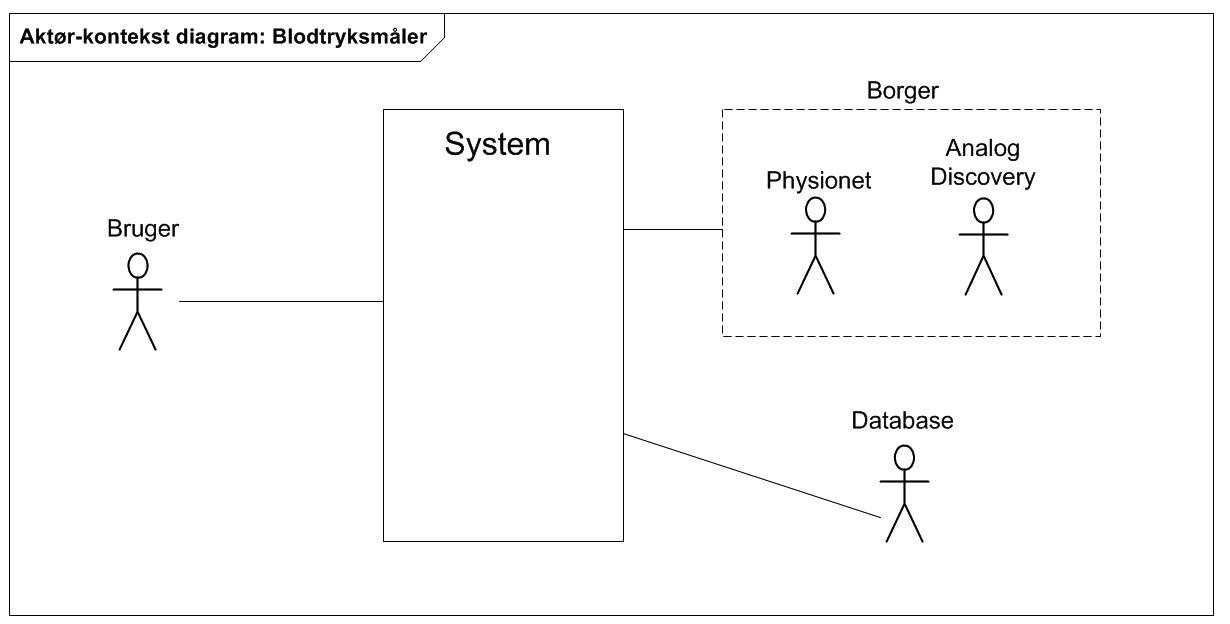
\includegraphics[width=1\textwidth]{Figurer/Snip20150929_7}
	\caption{Aktør-kontekstdiagram}
	\label{fig:aktoerbeskrivelse}
\end{figure}



\subsection{Aktørbeskrivelse}

\begin{table}[H]
\begin{tabularx}{\textwidth}{l X}
     Aktørnavn & Bruger \\
     Type & Primær \\
     Beskrivelse  & Person med relevant baggrundsviden inden for blodtryksanalyse \\ 
     \midrule
     Aktørnavn & Borger  \\
     Type & Sekundær \\
     Beskrivelse  & Borger er en kombination af Physionet og Analog Discovery. Borger repræsenterer data fra Physionet leveret til blodtryksmålingssystemet igennem Analog Discovery \\
     \midrule
     Aktørnavn & Database \\
     Type & Sekundær \\
     Beskrivelse  & Database bruges i blodtryksmålingssystemet til at gemme data \\ 
     \midrule
     Atørnavn & Physionet \\
     Type & Ekstern  \\
     Beskrivelse  & Physionet er en ekstern database, som indeholder blodtrykssignalet fra forskellige patienter \\
     \midrule
     Aktørnavn & Analog Discovery  \\
     Type & Ekstern \\
     Beskrivelse  & Analog Discovery omdanner data fra Physionet til at analogt signal \\                                                                                                                                                                          
     \bottomrule                                                                                                                   
    \end{tabularx}
    \caption {Aktørbeskrivelse}
    \label{tab:aktoerbeskrivelse}
	
\end{table}

\subsection{Use case-diagram}
\begin{figure}[H]
	\centering
	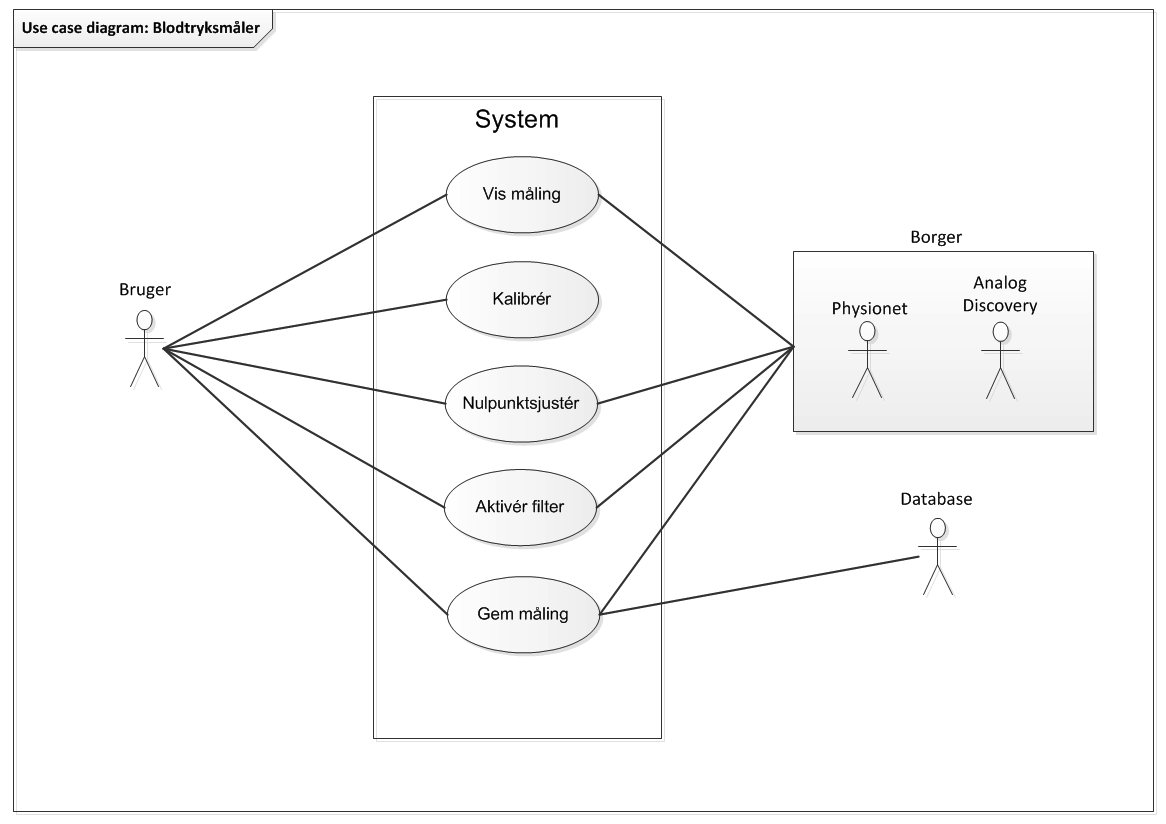
\includegraphics[width=1\textwidth]{Figurer/Snip20150929_8}
	\caption{Use case-diagram}
	\label{fig:Use case-diagram}
\end{figure}

\subsection{Use Cases}


\begin{longtabu} to \linewidth{@{}l r X[j]@{}} %UC1%
    {\large \textbf{Use Case 1}} && \\
    \toprule
    Navn &&    Vis Måling\\
    Use case ID &&    1\\
    Samtidige forløb &&    1\\
    Primær aktør &&    Bruger\\
    Sekundære aktør &&	 Borger\\
    Referencer &&    UC2 \\
    Mål &&    Bruger ønsker at vise blodtrykssignal uden digitalt filter\\
    Initiering &&	Startes af Bruger\\
    Forudsætninger &&  System er aktivt og tilgængeligt\\
    Resultat &&		Blodtrykssignalet udskrives                         \\ \midrule
    Hovedforløb &    1. &    Kalibrering-vinduet forekommer, hvor system spørger om der skal foretages en kalibrering\newline  
    						[1.a \textit{Bruger trykker på "Ja"\--knappen}]\newline
    						[1.b \textit{Bruger trykker på "Nej"\--knappen}]\\								
    			&    2. &    Blodtryksignal udskrives i Monitor-vinduet\newline\\ \midrule
                
    Undtagelser &    1.a &   Bruger ønsker kalibrering. UC2 gennemføres fra punkt 3 hvorefter UC1 fortsætter ved punkt 2\\[-1ex]
    			&	 1.b	 &	 Bruger ønsker ikke kalibrering. UC1 forsættes ved punkt 2   \\ \bottomrule
\caption{Fully dressed Use Case 1.}
\label{UC1}
\end{longtabu}


\begin{longtabu} to \linewidth{@{}l r X[j]@{}} %UC2%
    {\large \textbf{Use Case 2}} && \\
    \toprule
    Navn &&    Kalibrér\\
    Use case ID &&    2\\
    Samtidige forløb &&    1\\
    Primær aktør &&    Bruger\\
    Sekundære aktør &&	 \\
    Reference &&      \\
    Mål &&    Bruger ønsker at kalibrere blodtrykssignal\\
    Initiering &&	Startes af Bruger\\
    Forudsætninger &&  System er aktivt og tilgængeligt. UC1 kører\\
    Resultat &&		Blodtrykssignalet er kalibreret                         \\ \midrule
    Hovedforløb &    1. &	 Kalibrering-vinduet forekommer, hvor system spørger om der skal foretages en kalibrering\\[-1ex]  				
    			&    2. &    Bruger trykker på "Ja"\--knappen\newline
    						 [2.a \textit{Bruger trykker på "Nej"\--knappen}]\\
                &    3.	&	 System kalibrerer og udskriver, at kalibreringen er gennemført i kalibrerings-vinduet \newline\\ \midrule
                
    Undtagelser &    2.a &   Bruger ønsker ingen kalibrering. System fortsætter i UC1 ved punkt 2  \\ \bottomrule
\caption{Fully dressed Use Case 2.}
\label{UC2}
\end{longtabu}


\begin{longtabu} to \linewidth{@{}l r X[j]@{}} %UC3%
    {\large \textbf{Use Case 3}} && \\
    \toprule
    Navn &&    Nulpunktsjustér blodtrykssignal\\
    Use case ID &&    3\\
    Samtidige forløb &&    1\\
    Primær aktør &&    Bruger\\
    Sekundære aktør &&	Borger \\
    Reference &&      \\
    Mål &&    Bruger ønsker at nulpunktsjustere blodtrykssignal\\
    Initiering &&	Startes af Bruger\\
    Forudsætninger &&  System er aktivt og tilgængeligt. UC1 kører \\    Resultat &&		Blodtrykssignalet er nulpunktsjusteret\\ \midrule
    Hovedforløb &    1. &    Bruger trykker på "Nulpunktjustering"\--knappen og nulpunktsjustering starter\\[-1ex]   						 	
                &    2. &    System udskriver, at nulpunktsjustering er gemmenført i Monitor-vinduet\newline\\ \midrule
                
    Undtagelser &     &      \\ \bottomrule
\caption{Fully dressed Use Case 3.}
\label{UC3}
\end{longtabu}

\begin{longtabu} to \linewidth{@{}l r X[j]@{}} %UC4%
    {\large \textbf{Use Case 4}} && \\
    \toprule
    Navn &&    Aktivér digitalt filter\\
    Use case ID &&    4\\
    Samtidige forløb &&   1\\
    Primær aktør &&    Bruger\\
    Sekundære aktør &&	Borger \\
    Reference &&      \\
    Mål &&    Bruger ønsker at filtere blodtrykssignalet igennem et digitalt filter\\
    Initiering &&	Startes af Bruger\\
    Forudsætninger &&  System er aktivt og tilgængeligt. UC1 kører  \\
    Resultat &&		Digitalt filtreret blodtrykssignal udskrives i Monitor-vindet                 \\ \midrule
    Hovedforløb &    1. &    Bruger aktiverer filter ved at rykke switchen over på \textit{"Med digitalt filtre"} \\[-1ex]   						 	
                &    2. &    System udskriver at filteret er aktivt i Monitor-vinduet\newline\\ \midrule
                
    Undtagelser &     &      \\ \bottomrule
\caption{Fully dressed Use Case 4.}
\label{UC4}
\end{longtabu}

\begin{longtabu} to \linewidth{@{}l r X[j]@{}} %UC5%
    {\large \textbf{Use Case 5}} && \\
    \toprule
    Navn &&    Gem måling\\
    Use case ID &&    5\\
    Samtidige forløb &&   *\\
    Primær aktør &&    Bruger\\
    Sekundære aktør &&	Database \& Borger \\
    Reference &&      \\
    Mål &&    Bruger ønsker at gemme data i Database\\
    Initiering &&	Startes af Bruger\\
    Forudsætninger &&  System er aktivt og tilgængeligt. UC1 kører  \\
    Resultat &&		Data er gemt i Database                 \\ \midrule
    Hovedforløb &    1. &    Bruger trykker på "Gem"\--knappen \newline
       						 [1.a \textit{Borgerens data er gemt fra forrige målinger}]\\	
                &    2. &    System åbner Gem-vinduet\\[-1ex]
                &    3.	&	 Bruger indtaster data for blodtryksmålingen \\[-1ex]
                &	 4. &    Bruger trykker på "OK"\--knappen  \\[-1ex]
                &	 5.	&	 System lukker Gem-vinduet\\[-1ex]
                &	 6.	&	 System udskriver, at data er gemt i Monitor-vinduet\newline
                
                \\ \midrule
                
    Undtagelser &   1.a  &  UC5 forsættes ved UC5 ved punkt 6    \\ \bottomrule
\caption{Fully dressed Use Case 5.}
\label{UC5}
\end{longtabu}


\section{Ikke-funktionelle krav}


\subsection{(F)URPS+}
MoSCoW er angivet i parentes med hhv. M, S, C eller W.

\textbf{Usability}
\begin{itemize}
	\item (M) Brugeren skal kunne starte en default-måling maksimalt 20 sek. efter opstart af programmet
	\item (M) Login-vinduet skal indeholde en "login"\--knap til at logge på og få vist EKG-vinduet
	\item (M) EKG-vinduet skal indeholde en "start"\--knap til at igangsætte målingerne
	\item (M) EKG-vinduet skal indeholde en "log ud"\--knap
	\item (M) EKG-vinduet  skal indeholde en "gem"\--knap
	\item (M) Information-vinduet skal indeholde en "gem"\--knap
\end{itemize}

\textbf{Reliability}
\begin{itemize}
	\item (M) Systemet skal have en effektiv MTBF (Mean Time Between Failure) på 20 minutter og en MTTR (Mean Time To Restore) på 1 minut.
				\begin{align}
					Availability = \frac{MTBF}{MTBF+MTTR} = \frac{20}{20+1} = 0,952 = 95,2 \%
				\end{align}

\end{itemize}

\textbf{Performance}
\begin{itemize}
	\item (M) Der skal vises en EKG-graf i EKG-vinduet, hvor spænding vises op af y-aksen (-1V til 1V) og tiden på x-aksen
	\item (M) Grafen skal være scrollbar på x-aksen, så brugeren selv ved brug af musen kan vælge det udsnit af grafen, der skal vises mere detaljeret
	\item (M) Skal tage en sample over et brugerbestemt interval, hvor frekvensen  er tilpasset målingerne, således at grafen er analyserbar
\end{itemize}

\textbf{Supportability}
\begin{itemize}
	\item (M) Softwaren er opbygget af trelagsmodellen
\end{itemize}















